\chapter{Projektorganisation}
\subsection{Aufbau}
\subsubsection{}
Im Organigramm wird versuch, die klassischen Rollen eines Software-Projektes auf die Semesterabeit anzuwenden.

\begin{figure}[h]
	\centering
	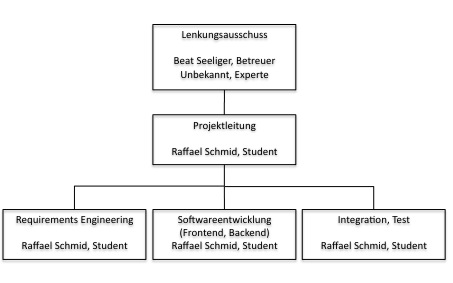
\includegraphics[height=8cm]{orgchart/Slide1}
	\caption[Organigramm]{Organigramm}
\end{figure}


\section{Rollen}
Die Semesterarbeit ist f\"ur den Rahmen eines strukturierten, professionellen Projektmanagements zu wenig umfangreich - normalerweise entspricht der zeitliche Aufwand von 120h dem Aufwand f\"ur Projektmanagement bei einem Mini-Projekt. Die Schwierigkeit bei der Strukturierung der Organisation und Rollen liegt darin, dass der Student mehrere Rollen - ausgenommen die des Kunden - selber \"ubernimmt. 

\subsection{Kunde, Auftraggeber}
Bei der Semesterarbeit geht es in erster Linie um das Erarbeiten von Wissen auf der Basis der Erstellung eines Prototypen f\"ur eine Ferienplanung. Die Idee stammt aus der Firma des Dozenten - der Kunde, Aufraggeber ist grunds\"atzlich fiktiv. 

\subsection{Requirements Engineer, Entwicklung, Tester}
Die Rollen des Requirements Engineers, Entwicklers, Testers werden alle vom Studenten \"ubernommen. Die sehr subektive Perspektive ist f\"ur das Endresultat ein Risiko.
